
\section{Cơ sở lý thuyết}

\textit{Chương 2 của luận văn tập trung vào việc trình bày các khái niệm cơ bản và lý thuyết nền tảng liên quan đến cơ sở dữ liệu phân tán, cụ thể là các hệ thống quản lý cơ sở dữ liệu như CockroachDB, TiDB, YugabyteDB, và Greenplum. Những cơ sở lý thuyết này đóng vai trò quan trọng trong việc hiểu rõ hơn về các vấn đề mà MSSQL đang gặp phải, cũng như cách thức mà các hệ thống phân tán có thể giải quyết các thách thức này.}

\textit{Phần đầu của chương giới thiệu về kiến trúc Shared-nothing, một kiến trúc phân tán trong đó mỗi node hoạt động độc lập, không chia sẻ tài nguyên với các node khác, từ đó tăng cường khả năng mở rộng và tính chịu lỗi. Chương này cũng đi sâu vào thuật toán Raft, một thuật toán đồng thuận phổ biến trong các hệ thống phân tán, giúp đảm bảo tính nhất quán của dữ liệu.}

Tiếp theo, chương này phân tích các hệ thống cơ sở dữ liệu phân tán hiện đại. Đầu tiên là CockroachDB với kiến trúc Shared-nothing, khả năng tự động cân bằng tải, và tối ưu hóa hiệu suất truy vấn. Sau đó, TiDB được giới thiệu với khả năng tương thích cao với MySQL, đồng thời cung cấp các tính năng nâng cao về khả năng chịu lỗi và mở rộng. YugabyteDB, một hệ thống quản lý cơ sở dữ liệu phân tán mã nguồn mở, được nhấn mạnh về khả năng kết hợp giữa SQL và NoSQL, cung cấp sự linh hoạt cao trong quản lý dữ liệu.

\textit{Phần cuối của chương tập trung vào Greenplum, hệ thống cơ sở dữ liệu phân tán được lựa chọn để thay thế MSSQL trong luận văn này. Chương trình bày chi tiết về kiến trúc của Greenplum, từ khả năng mở rộng ngang, xử lý song song, đến tính năng hỗ trợ OLTP và OLAP trên cùng một nền tảng. Kiến trúc MPP của Greenplum cho phép nó xử lý hiệu quả các dữ liệu lớn và phức tạp, đồng thời tích hợp các công cụ phân tích dữ liệu nâng cao.}

\textit{Chương này cũng trình bày một số tính năng và lợi ích của Greenplum, như khả năng mở rộng linh hoạt, tính ổn định và khả năng phân tích dữ liệu lớn, giúp lý giải vì sao Greenplum được chọn làm giải pháp thay thế trong nghiên cứu này.}

Việc chuyển đổi từ MSSQL sang các cơ sở dữ liệu phân tán không chỉ đơn giản là một bước chuyển giao công nghệ nó còn là việc áp dụng các phương pháp liên quan đã được chứng minh qua sự thành công của các giải pháp phân tán phổ biến như CockroachDB, TiDB, và YugabyteDB. Những giải pháp này không chỉ tăng cường khả năng mở rộng và hiệu suất mà còn cung cấp khả năng quản lý dữ liệu lớn và phức tạp một cách hiệu quả, đáp ứng nhu cầu ngày càng cao của các hệ thống quản lý thành viên trực tuyến ASP.NET Membership.

\subsection{Shared-nothing}

Thuật ngữ shared-nothing \cite{article} là một kiến trúc phân tán trong đó mỗi node trong hệ thống hoạt động độc lập và tự quản lý bộ nhớ cũng như các tài nguyên lưu trữ của chính nó, không có sự chia sẻ nào về bộ nhớ hoặc đĩa với các node khác. Đây là một mô hình phổ biến cho các cơ sở dữ liệu phân tán, hệ thống lưu trữ, và môi trường xử lý dữ liệu lớn vì nó giúp tăng khả năng mở rộng và khả năng chịu lỗi của hệ thống.

\begin{figure}
    \centering
    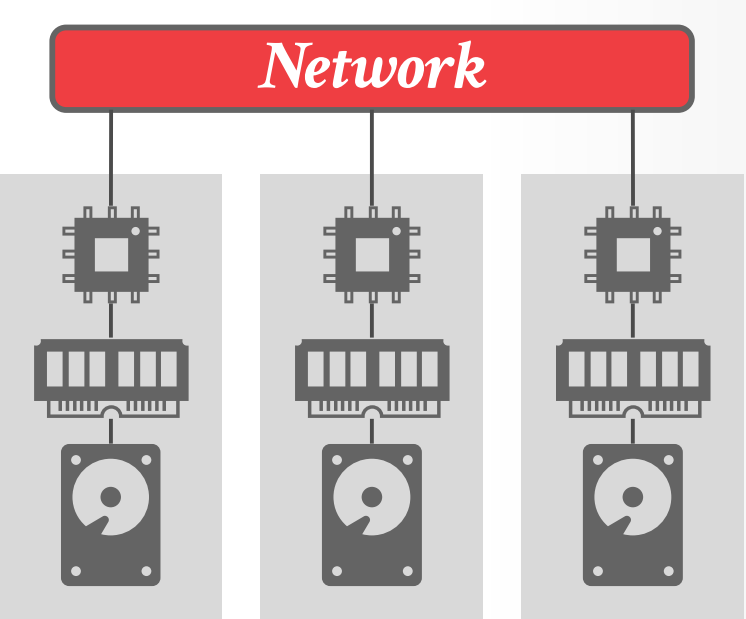
\includegraphics[width=1\linewidth]{ShareNothingAr.png}
    \caption{Kiến trúc Shared-nothing}
    \label{fig:ShareNothingAr}
\end{figure}

Hình \ref{fig:ShareNothingAr} minh họa kiến trúc shared-nothing với các node được kết nối thông qua một mạng lưới. Mỗi node được mô tả với một bộ vi xử lý (CPU), bộ nhớ (RAM) và ổ đĩa lưu trữ (Disk) riêng, nhấn mạnh sự độc lập của các tài nguyên và việc không có thành phần nào được chia sẻ giữa các node. Kết nối mạng cho thấy rằng mặc dù các node là một phần của cùng một hệ thống, chúng vẫn hoạt động độc lập, mỗi node xử lý dữ liệu và nhiệm vụ của riêng mình.

Đặc điểm chính của kiến trúc shared-nothing:

\textbf{Tính độc lập của node:} Mỗi node trong kiến trúc shared-nothing hoạt động độc lập. Nó quản lý CPU, bộ nhớ, và lưu trữ riêng của mình. Điều này loại bỏ các điểm nghẽn và phụ thuộc vào tài nguyên chung, cho phép hệ thống xử lý các yêu cầu một cách nhanh chóng và hiệu quả hơn.

\textbf{Khả năng mở rộng:} Vì mỗi node là độc lập, việc thêm node mới vào hệ thống là tương đối đơn giản và không làm ảnh hưởng đến hiệu suất của các node hiện tại. Điều này giúp kiến trúc shared-nothing có khả năng mở rộng cao, đặc biệt phù hợp với các ứng dụng lớn và phức tạp.

\textbf{Tăng khả năng chịu lỗi:} Trong kiến trúc shared-nothing, sự cố tại một node không ảnh hưởng trực tiếp đến các node khác. Điều này giúp hệ thống có khả năng chịu lỗi tốt hơn vì mỗi node có thể được thiết kế để có khả năng tự phục hồi hoặc chuyển đổi qua lại mà không cần sự can thiệp của các node khác.

\textbf{Tối ưu hóa hiệu suất:} Mỗi node có thể tối ưu hóa hiệu suất xử lý của riêng mình mà không bị ảnh hưởng bởi tải công việc hay yêu cầu xử lý tại các node khác. Điều này đặc biệt hữu ích trong các hệ thống xử lý dữ liệu lớn, nơi mà khối lượng công việc có thể được phân phối đều khắp các node.

\textbf{Quản lý dữ liệu:} Trong kiến trúc shared-nothing, dữ liệu thường được phân chia hoặc phân mảnh và được lưu trữ một cách độc lập trên từng node. Mỗi node có trách nhiệm quản lý và xử lý một phần của toàn bộ dữ liệu, điều này giúp giảm thiểu tắc nghẽn dữ liệu và tăng tốc độ truy vấn.

\subsection{Raft}

Raft \cite{ongaro2014raft} là một thuật toán đồng thuận được sử dụng trong các hệ thống phân tán để đảm bảo tính nhất quán của dữ liệu trên nhiều node. Raft giúp các node trong một cụm đồng ý về một trạng thái chung mặc dù có thể xảy ra sự cố hoặc mất mát thông tin. Thuật toán này được thiết kế để dễ hiểu và dễ triển khai hơn so với các thuật toán đồng thuận trước đây như Paxos.

Raft đạt được đồng thuận bằng cách phân chia quá trình thành ba thành phần chính: (1) Leader Election, trong đó các node bỏ phiếu để chọn ra một leader điều phối quá trình đồng thuận; (2) Log Replication nơi leader phân phối các lệnh (entries) nhật ký tới các node khác để sao chép; và (3) Safety đảm bảo các thay đổi được áp dụng một cách nhất quán trên tất cả các node.

Mỗi node trong Raft có thể ở một trong ba trạng thái: Leader, Follower, hoặc Candidate. Quá trình bầu cử xảy ra khi các node không nhận được thông tin từ Leader hiện tại, chuyển sang trạng thái Candidate và bắt đầu một cuộc bầu cử mới. Một khi Leader được bầu chọn, node đó sẽ quản lý tất cả các hoạt động sao chép nhật ký và đảm bảo sự đồng thuận trên cụm.

Raft đặc biệt hữu ích trong các hệ thống lưu trữ dữ liệu phân tán, cơ sở dữ liệu, và các ứng dụng yêu cầu độ tin cậy cao và tính nhất quán của dữ liệu.



\subsection{CockroachDB}

Trong thời đại kỹ thuật số ngày nay, nhu cầu về các hệ thống quản lý cơ sở dữ liệu đáp ứng được tính toàn cầu, độ tin cậy cao và khả năng mở rộng liên tục đang trở nên cấp thiết. CockroachDB \cite{taft2020cockroachdb}, được thiết kế với mục tiêu hỗ trợ các yêu cầu khắt khe này, là một hệ thống quản lý cơ sở dữ liệu thương mại phù hợp với các doanh nghiệp toàn cầu hiện đại. Đây là một giải pháp quản lý dữ liệu được tối ưu hóa để cung cấp khả năng chịu lỗi, hiệu suất cao.



CockroachDB triển khai một kiến trúc shared-nothing cho các cụm cơ sở dữ liệu. Điều này không chỉ cải thiện hiệu suất và khả năng mở rộng mà còn giúp tối ưu hóa quản lý tài nguyên. Trong một cụm CockroachDB, các node hoàn toàn ngang bằng nhau. Được lưu trữ trực tiếp trong node CockroachDB, mặc dù cũng có thể lưu trữ dữ liệu trên một hệ thống lưu trữ chia sẻ. Dữ liệu được phân phối trên cụm dựa trên các key ranges, mỗi range được sao chép tối thiểu ba lần trong cụm.

\begin{figure}
    \centering
    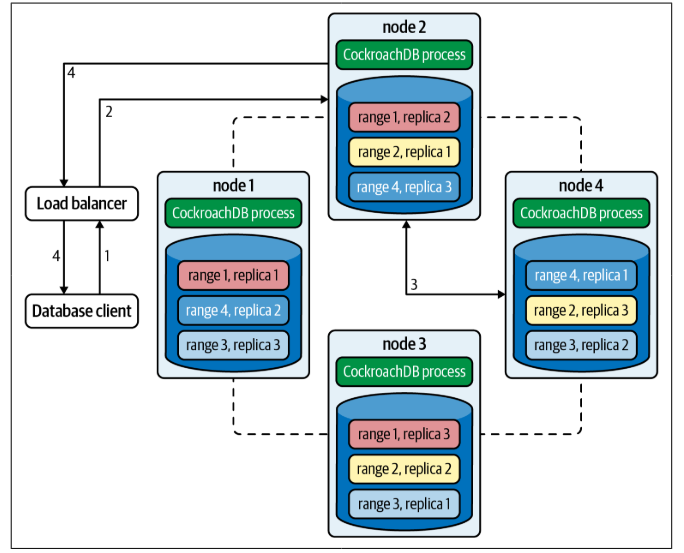
\includegraphics[width=0.8\linewidth]{CockroachdbArc.png}
    \caption{Kiến trúc một cụm trong CockroachDB \cite{CockroachDBGuide}}
    \label{fig:CockroachdbArc}
\end{figure}


Khi xét về cấu trúc cơ bản, một triển khai CockroachDB gồm nhiều quá trình máy chủ cơ sở dữ liệu. Mỗi máy chủ này được cấp phát lưu trữ độc lập, tuân theo mô hình cụm cơ sở dữ liệu shared-nothing. Điều này đồng nghĩa với việc mỗi node trong cụm CockroachDB hoạt động độc lập và không phụ thuộc vào node khác, không có sự phân biệt về vai trò giữa chính hay phụ. Lưu trữ này thường trực tiếp lưu trong máy chủ chạy dịch vụ CockroachDB, nhưng cũng có thể được cấu hình trên hệ thống lưu trữ chung. Dữ liệu được phân phối đều đặn qua cụm và có ít nhất ba bản sao được lưu trữ trên các máy chủ trong cụm.


Hình \ref{fig:layercrdb} minh họa cấu trúc các tầng của CockroachDB là một kiến trúc tầng phức tạp, mỗi tầng đóng một vai trò riêng biệt trong việc xử lý dữ liệu và yêu cầu.

\textbf{Tầng SQL}

Tầng SQL của CockroachDB là một thành phần cốt lõi, đóng vai trò cầu nối giữa người dùng và hệ thống cơ sở dữ liệu phân tán. Tầng này cho phép người dùng thực hiện các truy vấn và thao tác dữ liệu bằng ngôn ngữ SQL, một ngôn ngữ truy vấn chuẩn trong ngành được rất nhiều hệ quản trị cơ sở dữ liệu sử dụng.

Tầng SQL của CockroachDB tương thích cao với chuẩn SQL của PostgreSQL, điều này có nghĩa là nhiều ứng dụng được thiết kế cho PostgreSQL có thể chạy trên CockroachDB mà không cần chỉnh sửa lớn hoặc không chỉnh sửa. Sự tương thích này bao gồm hỗ trợ cho một loạt các tính năng SQL như truy vấn dữ liệu, các phép toán trên tập hợp, hàm tổng hợp, và giao dịch theo chuẩn ACID, cho phép người dùng thực hiện các truy vấn phức tạp và đa dạng.

Trong tầng SQL, truy vấn của người dùng được phân tích cú pháp và biên dịch thành một kế hoạch truy vấn. Quá trình này bao gồm việc xác định cách tốt nhất để thực hiện truy vấn dựa trên cấu trúc dữ liệu và các chỉ mục có sẵn. CockroachDB sử dụng một trình tối ưu hóa truy vấn mạnh mẽ để tạo ra kế hoạch hiệu quả nhất, giảm thiểu thời gian và tài nguyên cần thiết để trả về kết quả.


\textbf{Tầng Transaction}

Tầng Transaction đảm bảo tính toàn vẹn giao dịch theo nguyên tắc all or nothing, tức là tất cả các hoạt động trong một giao dịch phải hoàn thành hoàn toàn hoặc không được thực hiện. Cách tiếp cận này, với độ cô lập giao dịch mặc định là SERIALIZABLE—theo tiêu chuẩn ANSI SQL—đảm bảo rằng mỗi giao dịch diễn ra như thể nó được thực hiện trong một môi trường hoàn toàn độc lập.

\textbf{Tầng Distribution}

Distribution là một yếu tố quan trọng, giúp nền tảng này quản lý và phối hợp các hoạt động trên cụm dữ liệu phân tán. Đây là cách CockroachDB xử lý dữ liệu trên nhiều node một cách hiệu quả, bảo đảm tính sẵn sàng và nhất quán trong mọi giao dịch.

Đầu tiên, CockroachDB chia dữ các range, mỗi range có kích thước khoảng 128MB. Dữ liệu được phân tán tự động giữa các node trong cụm, nhằm mục đích cải thiện độ trễ và khả năng mở rộng. Mỗi range của dữ liệu không chỉ được lưu trữ tại một node mà còn được sao chép ra nhiều node khác, điều này đảm bảo độ bền và tính khả dụng cao của dữ liệu.

Để duy trì nhất quán dữ liệu trên toàn cụm, CockroachDB áp dụng giao thức Raft, đảm bảo rằng mọi thay đổi đối với dữ liệu đều được phản ánh một cách nhất quán trên tất cả các bản sao, giúp giảm thiểu lỗi và xung đột trong dữ liệu.

Bên cạnh việc sao chép, CockroachDB cũng sử dụng phân vùng dữ liệu để cải thiện hiệu suất truy vấn và cân bằng tải. Dữ liệu được phân bổ theo cách chiến lược trên các node để tối ưu hóa truy cập dữ liệu và quản lý tải truy cập hiệu quả, giảm độ trễ trong các truy vấn và tăng tốc độ xử lý.

Cuối cùng, CockroachDB có khả năng tự động cân bằng tải bằng cách liên tục điều chỉnh phân bổ dữ liệu giữa các node. Khi có sự thay đổi về tải truy cập hoặc dung lượng lưu trữ, hệ thống sẽ tự động chuyển dữ liệu giữa các node để duy trì hiệu quả hoạt động. Ngoài ra, trong trường hợp node gặp sự cố, CockroachDB có thể phục hồi nhanh chóng bằng cách tái tạo các bản sao range từ các node khác, giảm thiểu thời gian chết và bảo vệ dữ liệu.

\textbf{Tầng Replication}

Replication là một trong những thành phần chính giúp đảm bảo độ bền và tính khả dụng của dữ liệu trong một hệ thống phân tán. Tầng này quản lý việc sao chép dữ liệu giữa các node trong cụm, đảm bảo rằng dữ liệu luôn được bảo vệ và có thể truy cập ngay cả trong trường hợp sự cố.

Để quản lý và điều chỉnh việc phân bố ranges và sao chép, CockroachDB liên tục theo dõi và theo dõi tình trạng của các node. Hệ thống sử dụng thông tin này để tự động cân bằng lại dữ liệu giữa các node, tối ưu hóa hiệu suất và độ tin cậy. Khi một node mới được thêm vào cụm, CockroachDB có thể tự động sao chép và cân bằng ranges để tận dụng tài nguyên từ node mới, giảm bớt gánh nặng cho các node khác.

Khi một node bị lỗi, CockroachDB sẽ sử dụng các bản sao còn lại của dữ liệu để khôi phục lại range bị ảnh hưởng trên node khác. Quá trình này đảm bảo rằng cơ sở dữ liệu luôn khả dụng và dữ liệu không bị mất ngay cả khi xảy ra sự cố phần cứng.

\textbf{Tầng Storage}

Mỗi node trong CockroachDB chứa ít nhất một store, là đơn vị lưu trữ vật lý nơi dữ liệu được ghi và đọc từ đĩa. Mỗi store khởi tạo khi node bắt đầu hoạt động và chứa hai thành phần của Pebble engine: một dành cho dữ liệu tạm của các truy vấn SQL phân tán và một cho dữ liệu còn lại của node. Block cache được chia sẻ giữa tất cả các store trong node hỗ trợ cải thiện hiệu suất truy cập dữ liệu và phân phối thông minh dữ liệu giữa các stores, đảm bảo khả năng chịu lỗi và duy trì tính sẵn sàng cao của hệ thống.

Mỗi tầng trong kiến trúc CockroachDB được thiết kế để đáp ứng các yêu cầu kỹ thuật cụ thể, từ tối ưu hóa truy vấn đến đảm bảo độ tin cậy và sẵn sàng cao, đồng thời duy trì sự nhất quán và toàn vẹn dữ liệu trong môi trường phân tán.



\begin{figure}
    \centering
    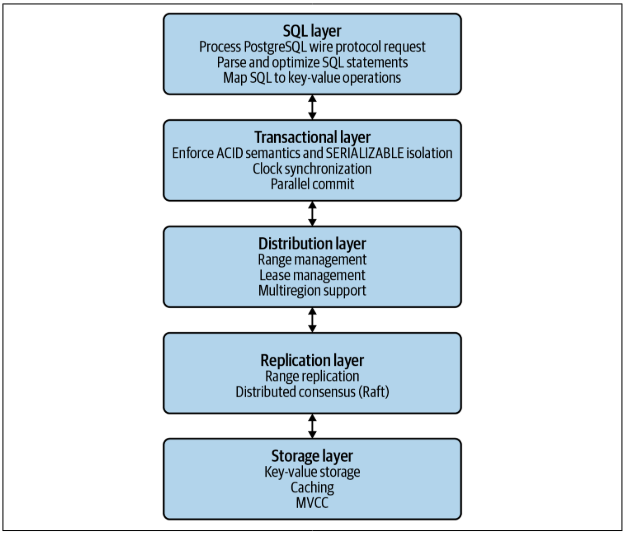
\includegraphics[width=0.8\linewidth]{layercrdb.png}
    \caption{Kiến trúc tầng trong CockroachDB \cite{CockroachDBGuide}}
    \label{fig:layercrdb}
\end{figure}


\subsection{TiDB}

TiDB \cite{huang2020tidb} là một hệ thống quản lý cơ sở dữ liệu phân tán được thiết kế để cung cấp khả năng tương thích cao với MySQL, đồng thời hỗ trợ các yêu cầu về khả năng chịu lỗi, độ tin cậy và mở rộng quy mô lớn. Kiến trúc của TiDB được thiết kế để tối ưu hóa cả hiệu suất giao dịch và truy vấn phân tích, làm cho nó trở thành một lựa chọn lý tưởng cho các doanh nghiệp cần một giải pháp cơ sở dữ liệu có khả năng phục vụ toàn cầu.

Kiến trúc TiDB gồm 3 thành phần chính là TiDB Server, Placement Driver server và Storage server như trinh hình \ref{fig:TiDBArchiteture}.


\begin{figure}
    \centering
    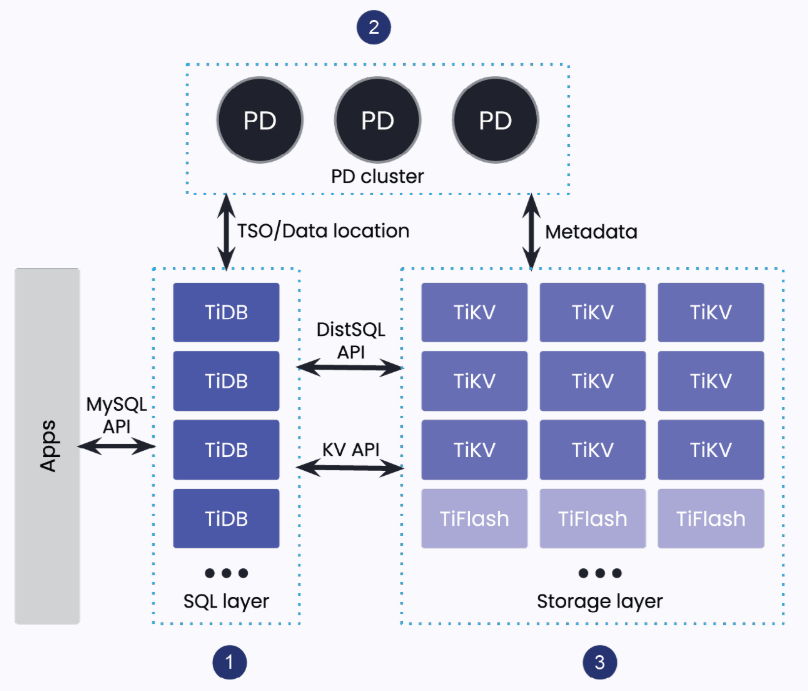
\includegraphics[width=0.6\linewidth]{TiDBArchiteture.png}
    \caption{Kiến trúc của TiDB\protect\footnotemark}
    \label{fig:TiDBArchiteture}
\end{figure}
\footnotetext{\url{https://static.pingcap.com/files/2024/02/01183648/TiDB_vs_MySQL_whitepaper.pdf}.}




\subsubsection{TiDB Server}

SQL Layer: Đây là lớp tiếp nhận các truy vấn SQL từ clients và chịu trách nhiệm phân tích cú pháp và tối ưu hóa các truy vấn. Lớp này hoạt động như một stateless server, có thể mở rộng ngang một cách dễ dàng bằng cách thêm các instances.

TiDB hỗ trợ giao thức MySQL, cho phép nó hoạt động và tích hợp một cách mượt mà với hầu hết các ứng dụng MySQL hiện có mà không cần chỉnh sửa.

\subsubsection{Placement Driver (PD) Layer}

Cluster Management: PD là thành phần quản lý tập trung của TiDB, chịu trách nhiệm cho việc lưu trữ metadata và quản lý và phân bổ dữ liệu giữa các TiKV nodes. PD cũng cân bằng tải và tối ưu hóa việc phân bổ dữ liệu trong cụm.

Scheduler: PD lên kế hoạch cho việc phân chia và sao chép dữ liệu, đảm bảo dữ liệu được sao chép và phân phối hợp lý giữa các nodes để cải thiện độ tin cậy và khả năng sẵn có.


\subsubsection{TiKV}

Storage Engine: TiKV là một engine lưu trữ phân tán, key-value, được xây dựng dựa trên thiết kế của Google Spanner. TiKV lưu trữ dữ liệu thực tế và xử lý các truy vấn dữ liệu cấp thấp từ TiDB layer.

Raft Consensus: TiKV sử dụng thuật toán đồng thuận Raft để đảm bảo tính nhất quán trong sao chép dữ liệu giữa các sao chép, từ đó nâng cao độ tin cậy của hệ thống.

Khả năng mở rộng theo chiều ngang: TiKV có thể mở rộng ngang một cách linh hoạt khi cần thêm tài nguyên, mà không gây ra gián đoạn.

\subsection{YugabyteDB}

\begin{figure}
    \centering
    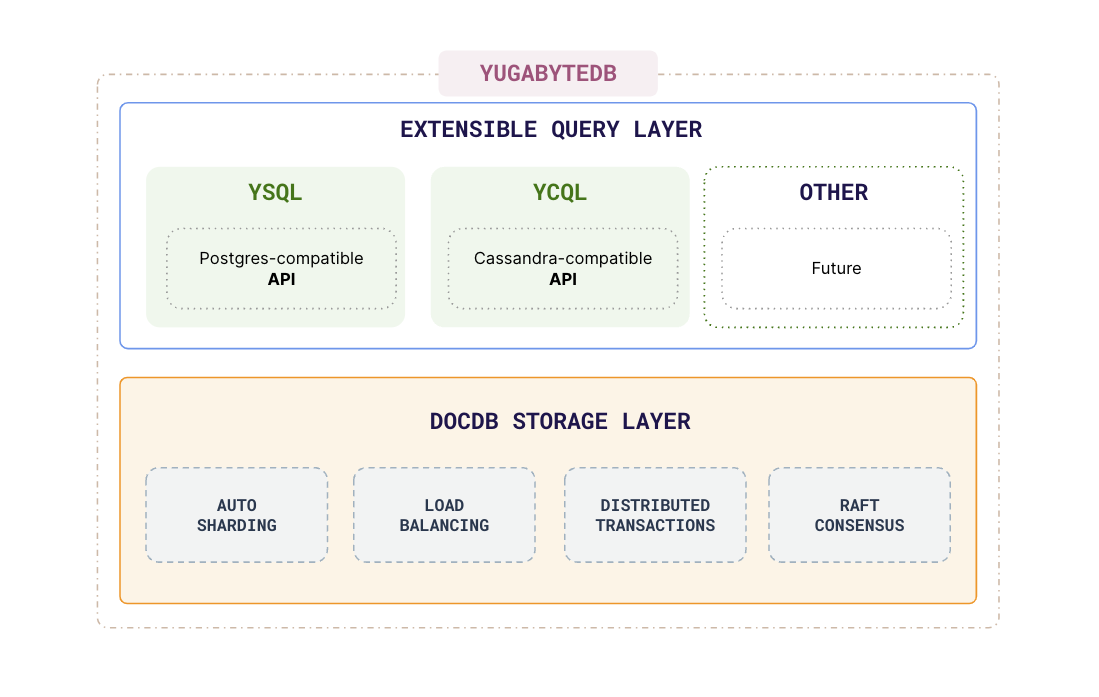
\includegraphics[width=0.8\linewidth]{YugaArchitecture.png}
    \caption{Kiến trúc của Yugabyte \protect\footnotemark}
    \label{fig:YugaArchitecture}
\end{figure}
\footnotetext{\url{https://docs.yugabyte.com/preview/architecture}.}



YugabyteDB là hệ thống quản lý cơ sở dữ liệu phân tán, mã nguồn mở, được thiết kế để đáp ứng nhu cầu về khả năng mở rộng cao và tính sẵn có liên tục cho các ứng dụng hiện đại. Với kiến trúc kết hợp linh hoạt giữa SQL và NoSQL, YugabyteDB mang lại sự đa dạng trong quản lý dữ liệu, tối ưu cho cả hai hình thức ứng dụng.

YugabyteDB bao gồm hai thành phần chính: YSQL và YCQL. YSQL là một lớp SQL hoàn chỉnh, tương thích với PostgreSQL, cho phép YugabyteDB hỗ trợ ứng dụng dựa trên SQL mà không cần chỉnh sửa. YCQL, ngược lại, là giao diện truy vấn dựa trên Apache Cassandra, được tối ưu hóa cho các hoạt động NoSQL với khả năng mở rộng cao và độ chịu lỗi tốt.

Sự đảm bảo về tính nhất quán của dữ liệu trên nhiều node trong cụm được hỗ trợ bởi thuật toán đồng thuận RAFT. Việc tổ chức dữ liệu thành các phân vùng, với mỗi phân vùng có thể có một hoặc nhiều bản sao, không chỉ củng cố độ tin cậy và khả năng chịu lỗi của hệ thống mà còn cải thiện hiệu suất đọc.

Hình \ref{fig:YugaArchitecture} mô tả kiến trúc của YugabyteDB được minh họa qua sự phân chia rõ ràng thành hai tầng cơ bản: tầng truy vấn và tầng lưu trữ. Tầng truy vấn, hoạt động như bộ não của hệ thống, chịu trách nhiệm xử lý yêu cầu của người dùng và điều hướng chúng tới vị trí dữ liệu thích hợp. Tầng này quan trọng trong việc giải mã và thực thi các lệnh SQL hoặc NoSQL tùy theo giao diện sử dụng: YSQL cho các tương tác giống SQL và YCQL cho các hoạt động NoSQL.

Tầng lưu trữ, đảm nhiệm việc quản lý vật lý dữ liệu, bảo đảm dữ liệu được lưu trữ một cách hiệu quả trên đĩa cứng. Tầng này quản lý các nhiệm vụ quan trọng như sao chép để bảo vệ dữ liệu khỏi mất mát và xử lý tính nhất quán để duy trì tính toàn vẹn của dữ liệu trên nhiều node. Ngoài ra, tầng lưu trữ sử dụng các thuật toán tiên tiến để tối ưu hóa quá trình truy xuất và lưu trữ dữ liệu, đảm bảo hiệu suất cao và độ bền trong các thao tác dữ liệu.

Các thành phần chính của YugabyteDB bao gồm:

\subsubsection{Storage Layer}

Storage Layer chịu trách nhiệm cho việc lưu giữ vật lý dữ liệu trên các thiết bị lưu trữ. Nó sử dụng DocDB, một hệ thống lưu trữ dạng key-value, được xây dựng dựa trên RocksDB, để quản lý hiệu quả việc lưu trữ và truy xuất dữ liệu. Thành phần này đảm bảo tính nhất quán và độ bền của dữ liệu thông qua cơ chế sao chép và phục hồi sau sự cố.

\subsubsection{Sharding}

Sharding trong YugabyteDB được thực hiện thông qua việc phân chia dữ liệu thành nhiều tablets, mỗi tablet là một khối dữ liệu độc lập được quản lý và phân bổ trên các node trong cụm. Điều này giúp cải thiện đáng kể khả năng mở rộng và hiệu suất truy xuất dữ liệu bằng cách phân tán tải và giảm thiểu điểm nghẽn.

\subsubsection{Replication}

Replication chịu trách nghiệm sao chép dữ liệu giữa các node được quản lý bởi thuật toán đồng thuận RAFT, đảm bảo tính nhất quán trong cụm. Mỗi tablet có một leader và nhiều followers, với leader chịu trách nhiệm xử lý các yêu cầu ghi và followers hỗ trợ đọc dữ liệu, từ đó cải thiện khả năng chịu lỗi và độ sẵn sàng của hệ thống.

\subsubsection{Transactions}

YugabyteDB hỗ trợ giao dịch đa bảng với đảm bảo tính toàn vẹn dữ liệu theo mô hình ACID. Cơ chế giao dịch này được xây dựng dựa trên cơ sở của snapshot isolation, cho phép các giao dịch song song diễn ra mà không ảnh hưởng lẫn nhau, đảm bảo hiệu suất và tính nhất quán cao.

\subsubsection{Master Server}
Master Server trong YugabyteDB chịu trách nhiệm quản lý toàn bộ metadata của cụm, bao gồm cấu hình cụm, schema của các bảng và trạng thái của các tablets. Nó cũng phụ trách việc cân bằng tải và phân bổ tài nguyên giữa các node, giúp tối ưu hóa hiệu suất và khả năng phục hồi.

\subsubsection{TServer (Tablet Server)}

TServer là nơi xử lý trực tiếp các yêu cầu đọc và ghi dữ liệu trên các tablets mà nó quản lý. Mỗi TServer chịu trách nhiệm cho một nhóm các tablets, thực hiện các thao tác dữ liệu và phối hợp với các TServer khác cùng với Master Server để đảm bảo hoạt động ổn định và hiệu quả của hệ thống.

Các thành phần này, khi làm việc cùng nhau, tạo nên một hệ thống cơ sở dữ liệu mạnh mẽ, linh hoạt, và đáng tin cậy, đáp ứng nhu cầu của các ứng dụng quan trọng trong thời đại số hiện nay.

Với những cải tiến này, YugabyteDB đem lại một giải pháp cơ sở dữ liệu mạnh mẽ, đáp ứng nhu cầu về hiệu suất cao, khả năng mở rộng và tính sẵn sàng cao cho các ứng dụng quan trọng trong thời đại số.

\subsection{Greenplum}


Greenplum \cite{lyu2021Greenplum} là một hệ thống quản lý cơ sở dữ liệu phân tán, được thiết kế đặc biệt để xử lý và phân tích dữ liệu lớn (big data). Phát triển dựa trên nền tảng PostgreSQL, hệ thống này tận dụng khả năng mở rộng và tính năng xử lý song song, cung cấp một giải pháp mạnh mẽ và linh hoạt cho các doanh nghiệp cần xử lý khối lượng dữ liệu khổng lồ.

Một trong những điểm nổi bật của Greenplum là khả năng mở rộng ngang. Điều này cho phép hệ thống tăng thêm năng lực xử lý và lưu trữ mà không cần đầu tư lớn vào cơ sở hạ tầng. Với kiến trúc phân tán, Greenplum có thể dễ dàng thêm các node mới mà không gây gián đoạn hoạt động. Điều này đảm bảo khả năng phản ứng nhanh chóng với sự tăng trưởng đột ngột của dữ liệu, giúp các tổ chức duy trì hoạt động ổn định và hiệu quả.

Greenplum được xây dựng dựa trên kiến trúc xử lý song song đại trà (Massively Parallel Processing - MPP). Kiến trúc này cho phép nhiều bộ vi xử lý thực hiện tác vụ độc lập nhưng đồng thời, giúp xử lý hiệu quả các dữ liệu lớn và phức tạp. Điều này được thực hiện qua các segment độc lập, mỗi segment xử lý một phần dữ liệu, từ đó cắt giảm độ trễ và tối đa hóa hiệu suất khi thực hiện các truy vấn phức tạp.

Greenplum được tối ưu hóa để hỗ trợ cả xử lý giao dịch trực tuyến (Online Transaction Processing - OLTP) và xử lý phân tích trực tuyến (Online Analytical Processing - OLAP) trên cùng một hệ thống. Sự tích hợp này giúp giảm thiểu sự phức tạp trong cơ sở dữ liệu và tiết kiệm chi phí bằng cách loại bỏ nhu cầu duy trì nhiều hệ thống riêng biệt. Greenplum sử dụng giao thức cam kết một pha (One-Phase Commit Protocol) cho các giao dịch chỉ liên quan đến một segment duy nhất, giúp cải thiện hiệu suất và giảm thời gian đáp ứng cho các truy vấn OLTP.

Ngoài các truy vấn SQL cơ bản, Greenplum còn cung cấp các công cụ phân tích dữ liệu nâng cao như học máy và xử lý dữ liệu lớn. Những công cụ này giúp đơn giản hóa và hiệu quả hóa việc phân tích dữ liệu phức tạp, giúp tổ chức trích xuất giá trị tối đa từ dữ liệu lớn. Điều này đặc biệt quan trọng trong bối cảnh các doanh nghiệp ngày càng phải đối mặt với khối lượng dữ liệu ngày một tăng và yêu cầu phân tích ngày càng phức tạp.

Tổng hợp lại, Greenplum là một giải pháp quản lý dữ liệu đa năng, hiệu quả và linh hoạt, phù hợp cho cả hoạt động xử lý giao dịch hàng ngày và các tác vụ phân tích dữ liệu sâu rộng. Khả năng mở rộng ngang của hệ thống cho phép dễ dàng thêm các node mới vào cụm mà không gây gián đoạn dịch vụ hiện hữu. Điều này đặc biệt quan trọng khi cần xử lý khối lượng dữ liệu tăng lên một cách nhanh chóng và hiệu quả, giúp các tổ chức duy trì tính cạnh tranh và đáp ứng nhu cầu phát triển không ngừng của thị trường.

\subsubsection{Kiến trúc của Greenplum}

Greenplum với mỗi node có hiệu suất tương đương cơ sở dữ liệu MPP kiến trúc của hệ thống. Hình \ref{fig:gp-architecture} mô tả kiến trúc của Greenplum.

\begin{figure}[htbp]
\centerline{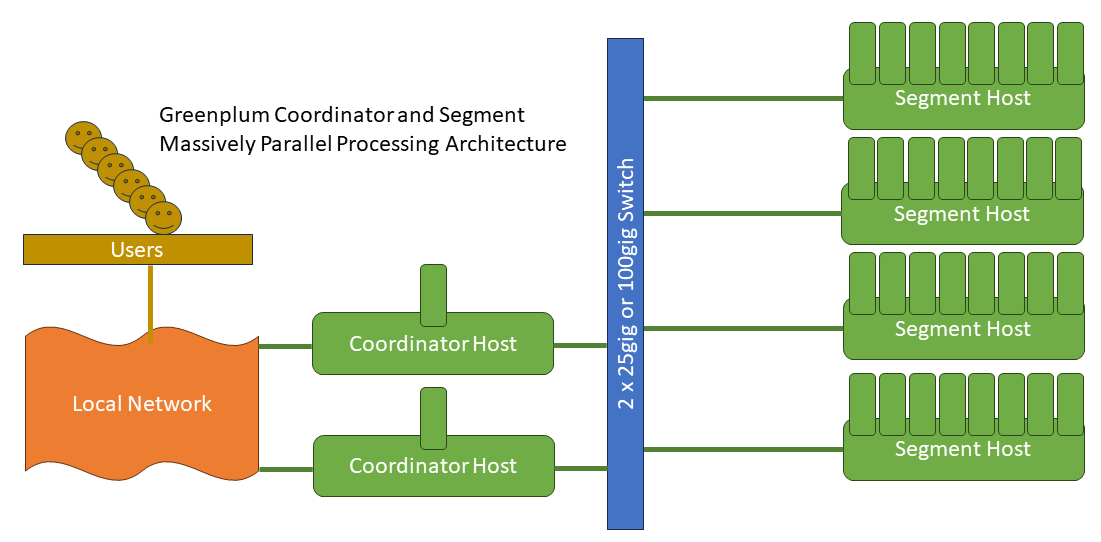
\includegraphics[scale=.4]{gp-architecture.png}}
\captionsetup{font=Large}
\caption{Kiến trúc hệ thống cơ sở dữ liệu Greenplum\protect\footnotemark.  }
\label{fig:gp-architecture}
\end{figure}
\footnotetext{\url{https://docs.vmware.com/en/VMware-Greenplum/7/greenplum-database/admin_guide-intro-arch_overview.html}.}


Greenplum là hệ thống cơ sở dữ liệu được xây dựng dựa trên kiến
trúc MPP, được tối ưu hóa để xử lý dữ liệu lớn và phân tích.


\paragraph{Coordinator}

Coordinator trong kiến trúc Greenplum là nơi quản lý và điều phối
toàn bộ hoạt động của cơ sở dữ liệu. Hình \ref{fig:admin_guide-graphics-standby_coordinator} Mô tả coordinator trong kiến trúc Greenplum.
Dưới đây là các yếu tố cụ thể:


\begin{figure}[htbp]
\centerline{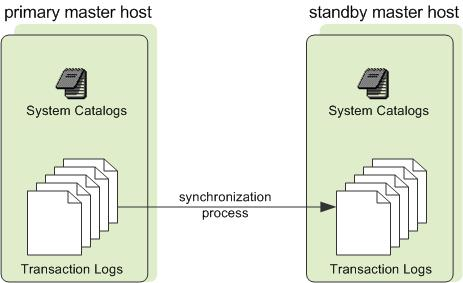
\includegraphics[scale=.7]{admin_guide-graphics-standby_coordinator.jpg}}
\captionsetup{font=Large}
\caption{Coordinator trong kiến trúc Greenplum \protect\footnotemark}
\label{fig:admin_guide-graphics-standby_coordinator}
\end{figure}
\footnotetext{\url{https://docs.vmware.com/en/VMware-Greenplum/7/greenplum-database/admin_guide-intro-arch_overview.html}.}

\textbf{Quản lý truy vấn và điều phối:} Coordinator nhận các truy vấn từ ứng dụng người dùng và chịu trách nhiệm phân tích cú pháp, tối ưu hóa truy vấn, và lập kế hoạch thực thi truy vấn. Nó phân phối các phần của truy vấn đã được tối ưu hóa đến các segment nodes để thực hiện.


\textbf{Duy trì Metadata:} Coordinator duy trì danh mục (catalog) của cơ sở dữ liệu, nơi lưu giữ thông tin về sơ đồ, dữ liệu, và cấu trúc của các bảng, cũng như các thông tin thống kê cần thiết cho việc tối ưu hóa truy vấn.

\textbf{Quản lý giao dịch:} Coordinator xử lý và quản lý các giao dịch, đảm bảo tính toàn vẹn, nhất quán, và cô lập dữ liệu. Nó sử dụng giao thức cam kết hai pha (two-phase commit protocol) để đảm bảo các thay đổi được thực hiện một cách đồng nhất trên tất cả các segment nodes.


\textbf{Quản lý Tài nguyên:} Coordinator quản lý các nguồn tài nguyên như bộ nhớ và CPU cho các truy vấn và có thể thiết lập các ưu tiên dựa trên chính sách quản lý tài nguyên.

\textbf{Phục hồi và Sao lưu:} Trong trường hợp có sự cố, master host có trách nhiệm khởi tạo các quy trình sao lưu và phục hồi để bảo đảm tính sẵn sàng và liên tục của hệ thống.

\textbf{Monitoring và Logging:} Coordinator cũng có trách nhiệm giám sát hoạt động của cả hệ thống và ghi lại các sự kiện hệ thống, giúp trong việc phân tích hiệu suất và khắc phục sự cố. Coordinator đóng vai trò trung tâm trong kiến trúc Greenplum, đảm nhiệm nhiều chức năng quan trọng từ việc quản lý truy vấn đến quản lý tài nguyên và đảm bảo tính ổn định của hệ thống.

\paragraph{Segment}

Trong kiến trúc Greenplum, segment là những máy chủ cơ sở dữ liệu hoặc
nodes làm việc song song để xử lý và lưu trữ dữ liệu. Dưới đây là mô tả chi tiết về segment trong Greenplum:

\textbf{Xử lý dữ liệu song song:} Mỗi segment là một node xử lý độc lập, chạy một instance của cơ sở dữ liệu PostgreSQL. Các segment làm việc cùng nhau một cách song song, mỗi segment xử lý một phần của truy vấn tổng thể và dữ liệu liên quan.

\textbf{Lưu trữ phân tán:} Dữ liệu trong Greenplum được phân phối đều ra các segment. Mỗi segment chứa một phần dữ liệu và được quản lý độc lập.
Kỹ thuật phân phối có thể bao gồm hash-based, random, hoặc các phân vùng
dữ liệu cụ thể. 

\textbf{Tính độc lập và kiến trúc shared-nothing:}
Mỗi segment có bộ nhớ và không gian lưu trữ của riêng mình, tuân theo kiến trúc shared-nothing. Điều này đảm bảo rằng không có sự phụ thuộc giữa các segment, giảm thiểu các điểm nghẽn và cải thiện hiệu suất.

\textbf{Tự động phục hồi:} Greenplum có khả năng tự động phục hồi từ lỗi ở cấp segment. Khi một segment gặp sự cố, Greenplum có thể chuyển công việc sang một segment dự bị hoặc phục hồi segment bị lỗi.

\textbf{Hiệu suất cao và khả năng mở rộng:} Do mỗi segment xử lý một phần nhỏ của dữ liệu, hệ thống có thể mở rộng quy mô một cách linh hoạt bằng cách thêm segment vào hệ thống để xử lý khối lượng dữ liệu lớn hơn.
Sự mở rộng này có thể được thực hiện mà không cần thay đổi cấu trúc hoặc
cấu hình của các segment hiện có.

\textbf{Quản lý và giám sát:}
Mỗi segment được giám sát bởi coordinator, đảm bảo rằng nó hoạt động đúng
và hiệu quả. Coordinator có thể giám sát tình trạng và hiệu suất của từng segment, và thực hiện các điều chỉnh khi cần thiết.

\textbf{Cân bằng tải:} Greenplum sử dụng cơ chế cân bằng tải để đảm bảo rằng không có segment nào bị quá tải hoặc nhàn rỗi.
Việc phân phối công việc giữa các segment được thực hiện dựa trên cấu hình và tình trạng hiện tại của hệ thống.

Segments đóng vai trò quan trọng trong việc đảm bảo khả năng xử lý dữ liệu lớn và phức tạp của Greenplum, giúp nó trở thành một giải pháp mạnh mẽ cho việc kho dữ liệu và phân tích dữ liệu quy mô lớn.

\paragraph{Node Motion}

Greenplum đã giới thiệu một node kế hoạch mới có tên là Motion để thực hiện việc di chuyển dữ liệu này. Node Motion sử dụng mạng để gửi và nhận dữ liệu từ các segment khác nhau, tạo điều kiện cho việc phân chia kế hoạch truy vấn thành nhiều phần khác nhau, mỗi phần được gọi là một slice. Mỗi slice sau đó được thực thi bởi một nhóm các quá trình phân tán, được gọi chung là gang. Với việc sử dụng node Motion và khái niệm gang, kế hoạch truy vấn và quá trình thực thi của Greenplum trở nên phân tán. Kế hoạch sẽ được gửi đến từng quá trình, và mỗi quá trình sẽ thực thi phần slice của kế hoạch dựa trên ngữ cảnh và trạng thái cục bộ của mình. Điều này phản ánh kỹ thuật Single Program Multiple Data (SPMD), nơi cùng một kế hoạch được phân phát đến các nhóm quá trình trên khắp cụm. Các quá trình khác nhau được tạo ra bởi các segment khác nhau sẽ có ngữ cảnh, trạng thái và dữ liệu cục bộ riêng của chúng. Hình \ref{fig:plan} ví dụ về kế hoạch phân tán và thực thi của Greenplum.

\begin{figure}[htbp]
\centerline{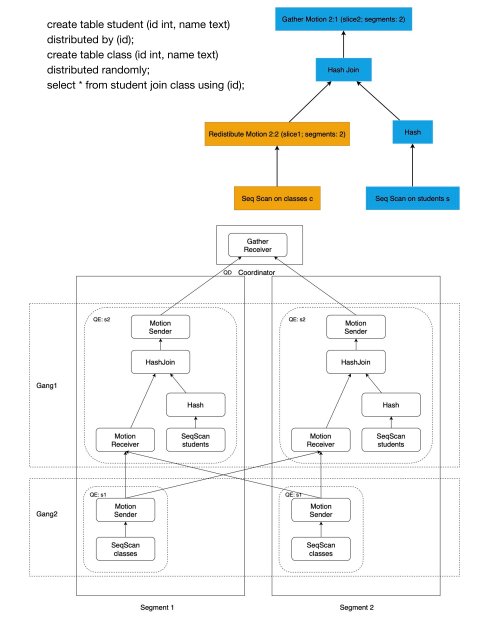
\includegraphics[scale=1]{plan.PNG}}
\captionsetup{font=Large}
\caption{Kế hoạch phân tán và thực thi của Greenplum \cite{lyu2021Greenplum}}
\label{fig:plan}
\end{figure}

Từ hình \ref{fig:plan} cho thấy Greenplum bảng student được tạo với việc phân phối dữ liệu dựa trên cột id. Điều này có nghĩa là dữ liệu sẽ được phân chia giữa các segment sao cho mỗi id student sẽ chỉ tồn tại trên một segment cụ thể. Bảng class được tạo với dữ liệu phân phối một cách ngẫu nhiên, không theo một quy tắc cụ thể nào. Khi truy vấn SELECT * FROM student JOIN class USING (id); được thực hiện, hệ thống sẽ tạo ra một kế hoạch thực thi phân tán. Kế hoạch này xác định làm thế nào dữ liệu từ cả hai bảng sẽ được kết hợp dựa trên cột id. Các segment thực hiện quét tuần tự (Seq Scan) trên bảng student và class để lấy các bản ghi cần thiết cho việc thực hiện join. Motion Sender: Nằm trên mỗi Motion Sender: Nằm trên mỗi segment, sẽ xác định các bản ghi từ bảng
class mà cần được di chuyển để join với bảng student.
Motion Receiver nằm trên segment đích, sẽ nhận các bản ghi từ bảng class
đã được gửi qua và chuẩn bị cho việc join, sẽ xác định các bản ghi từ bảng class mà cần được di chuyển để join với bảng student. Motion Receiver nằm trên segment đích, sẽ nhận các bản ghi từ bảng class đã được gửi qua và chuẩn bị cho việc join. Trong mỗi segment, một Hash Join được thực hiện giữa các bản ghi từ bảng student và các bản ghi từ bảng class đã được di chuyển đến. Đây là bước dữ liệu từ bảng class có thể cần được phân phối lại (redistributed) giữa các segment để đảm bảo rằng mỗi student có thể được join với đúng class dựa trên id. Sau khi join được thực hiện trên các segment, kết quả sau cùng sẽ được gửi về cho Gather Receiver ở coordinator, nơi tất cả kết quả từ các segment được tổng hợp lại. Coordinator sau đó sẽ trả về kết quả cuối cùng của truy vấn join cho người dùng hoặc ứng dụng đã yêu cầu truy vấn. Trong quá trình này, Gang1 và Gang2 có thể hiểu là nhóm các quá trình làm việc trên các segment khác nhau để thực hiện các phần khác nhau của kế hoạch thực thi (ví dụ: quét tuần tự, join). Mỗi gang có thể gồm nhiều slice, tương ứng với một phần của công việc cần thực hiện trên mỗi phân
đoạn.

\paragraph{Orca: Tối ưu hóa truy vấn trong Greenplum}



Orca \cite{orca} là một hệ thống tối ưu hóa truy vấn hiện đại, được thiết kế để cải thiện hiệu suất xử lý truy vấn trong các hệ thống dữ liệu lớn, bao gồm Greenplum. Orca hoạt động bằng cách tạo ra các kế hoạch truy vấn tối ưu, tối ưu hóa thứ tự kết hợp (join ordering), loại bỏ phân vùng không cần thiết (partition elimination), và sử dụng nhiều kỹ thuật khác để giảm thiểu chi phí và thời gian xử lý truy vấn.


Orca được xây dựng với một kiến trúc mô-đun hiện đại, được tối ưu hóa cho việc xử lý dữ liệu lớn trong môi trường phân tán. Hình \ref{fig:architect-orca} dưới đây minh họa kiến trúc của Orca, cho thấy cách các thành phần chính trong hệ thống tương tác với nhau để tối ưu hóa truy vấn SQL.


Ở lớp trên cùng của Orca, các thành phần chính bao gồm Search, Job Scheduler, và Memo. Search chịu trách nhiệm tìm kiếm và xác định các kế hoạch truy vấn khả thi. Job Scheduler quản lý và điều phối việc thực thi các nhiệm vụ tối ưu hóa, đảm bảo các bước trong quá trình tối ưu hóa được thực hiện đúng thứ tự và đúng thời gian. Memo là một cấu trúc dữ liệu nội bộ, lưu trữ các kế hoạch truy vấn khả thi và các thông tin liên quan, giúp giảm thiểu việc tính toán lại và tăng hiệu quả của quá trình tối ưu hóa.


Bên cạnh đó, Orca còn có Optimizer Tools, một tập hợp các công cụ tối ưu hóa mạnh mẽ, bao gồm các thành phần như Operators, Property Enforcement, Transformations, Cardinality Estimation, Cost Model, và MD Cache. Sự phối hợp chặt chẽ giữa các thành phần này đảm bảo hiệu suất truy vấn tối ưu.

Operators đại diện cho các phép toán cần thực hiện trên dữ liệu như phép nối (join), phép lọc (filter), tổng hợp (aggregate), và sắp xếp (sort).
Property Enforcement đảm bảo rằng các kế hoạch truy vấn tuân thủ các thuộc tính cần thiết, chẳng hạn như thứ tự sắp xếp và chỉ mục, để đảm bảo tính chính xác và hiệu quả của quá trình thực thi.
Transformations áp dụng các quy tắc và thuật toán để tạo ra nhiều phiên bản tối ưu khác nhau của một kế hoạch truy vấn, từ đó lựa chọn phiên bản tốt nhất.
Cardinality Estimation giúp ước tính số lượng bản ghi mà mỗi toán tử sẽ xử lý, cung cấp thông tin quan trọng cho việc xây dựng kế hoạch truy vấn chính xác.
Cost Model đánh giá và so sánh các kế hoạch truy vấn dựa trên chi phí tài nguyên hệ thống, bao gồm CPU, I/O, bộ nhớ và thời gian xử lý, để lựa chọn kế hoạch tối ưu nhất.
MD Cache lưu trữ siêu dữ liệu về các đối tượng trong cơ sở dữ liệu, cho phép truy cập nhanh chóng thông tin cần thiết trong quá trình tối ưu hóa.
Quy trình tương tác với hệ thống cơ sở dữ liệu

Orca hoạt động dựa trên nền tảng GPOS (Generic Portable Operating System Layer), cung cấp các chức năng hệ điều hành cơ bản như quản lý nhập/xuất tệp, xử lý ngoại lệ, quản lý tính đồng thời, và quản lý bộ nhớ. Hình \ref{fig:interac-orca} mô tả quy trình tương tác của Orca với hệ thống cơ sở dữ liệu:


Quá trình tương tác giữa Orca và hệ thống cơ sở dữ liệu Greenplum bắt đầu khi một truy vấn SQL được gửi đến. Đầu tiên, Parser, một thành phần phân tích cú pháp, sẽ tiếp nhận truy vấn này và chuyển đổi nó thành một biểu diễn trung gian gọi là DXL (Data eXchange Language). DXL đóng vai trò như một ngôn ngữ chung, cho phép Orca giao tiếp và xử lý truy vấn một cách hiệu quả.

Sau khi truy vấn được chuyển đổi thành DXL, Orca sẽ thực hiện quá trình tối ưu hóa phức tạp. Optimizer trong Orca sử dụng các kỹ thuật tiên tiến như tối ưu hóa thứ tự kết hợp (join ordering), loại bỏ phân vùng không cần thiết (partition elimination), và nhiều kỹ thuật khác để phân tích và tìm ra kế hoạch thực thi truy vấn tối ưu nhất. Kế hoạch này, được gọi là DXL Plan, chi tiết các bước cần thiết để thực thi truy vấn một cách hiệu quả nhất, bao gồm cả việc điều phối và di chuyển dữ liệu giữa các node trong hệ thống phân tán Greenplum.

Executor sau đó sẽ nhận DXL Plan từ Orca và tiến hành thực thi kế hoạch này. Trong quá trình thực thi, Executor sẽ tương tác với các thành phần khác của Greenplum, bao gồm cả Node Motion, để điều phối việc di chuyển dữ liệu giữa các node một cách hiệu quả. Node Motion là một quá trình quan trọng trong Greenplum, đảm bảo rằng dữ liệu được phân phối và xử lý một cách tối ưu trên toàn bộ hệ thống phân tán. Orca, với khả năng tối ưu hóa vượt trội, giúp cải thiện hiệu suất của Node Motion, từ đó tăng tốc độ xử lý truy vấn và giảm thiểu chi phí.

Cuối cùng, sau khi Executor hoàn thành việc thực thi kế hoạch truy vấn, kết quả sẽ được trả về cho người dùng. Nhờ sự phối hợp chặt chẽ giữa các thành phần của Orca và Greenplum, quá trình xử lý truy vấn trở nên hiệu quả và tối ưu hơn, đặc biệt là khi xử lý khối lượng lớn dữ liệu trong môi trường phân tán.

\begin{figure}
    \centering
    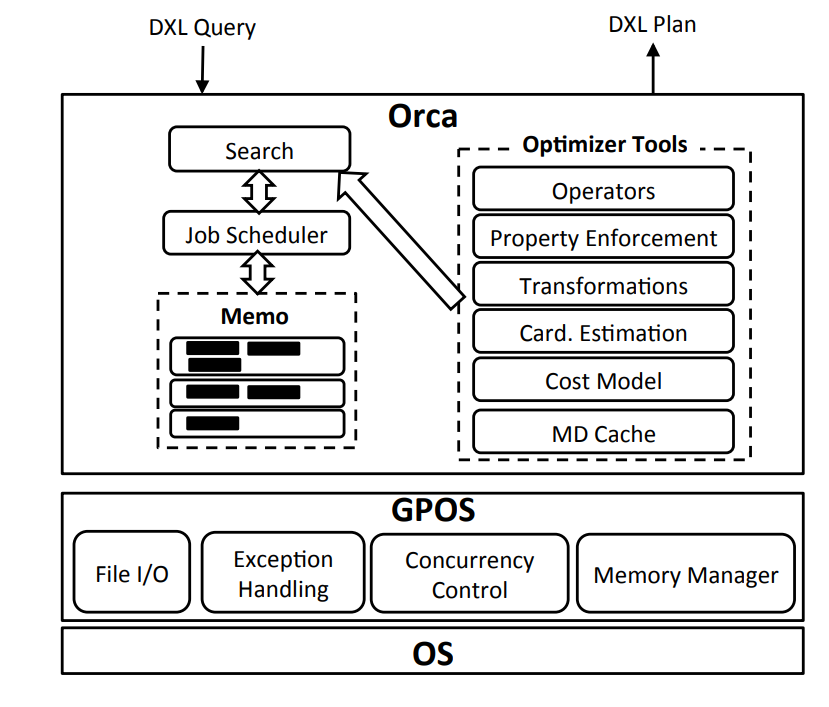
\includegraphics[width=1\linewidth]{architect-orca.png}
    \caption{Kiến trúc tổng quát của orca \cite{orca}}
    \label{fig:architect-orca}
\end{figure}


\begin{figure}
    \centering
    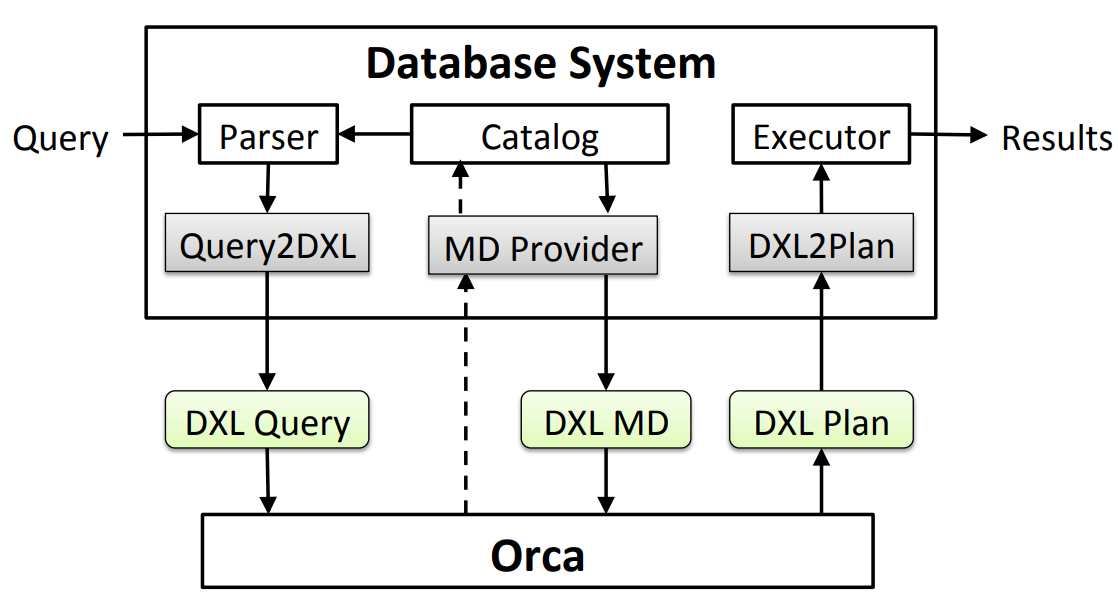
\includegraphics[width=1\linewidth]{interac-orca.png}
    \caption{Tương tác Orca với Greenplum \cite{orca}}
    \label{fig:interac-orca}
\end{figure}



\paragraph{Khóa}

Trong Greenplum, khóa được sử dụng rộng rãi để ngăn chặn các tình huống
đua tranh ở nhiều cấp độ khác nhau. Có ba loại khóa khác nhau được thiết kế cho các trường hợp sử dụng khác nhau: khóa quay vòng (spin locks), khóa nhẹ (LWlocks), và khóa đối tượng (Object locks).

Khóa quay vòng là loại khóa cực kỳ đơn giản, thường được sử dụng để bảo
vệ các cấu trúc dữ liệu nhỏ và đơn giản. Khi một tiến trình cần truy cập vào một tài nguyên được bảo vệ bởi một spin lock, nó sẽ liên tục kiểm tra (hay quay vòng) để xem khóa có sẵn hay không. Nếu khóa không sẵn có, tiến trình sẽ tiếp tục vòng lặp này cho đến khi nó có thể giành được khóa. Spin locks phù hợp khi thời gian giữ khóa ngắn, vì nó yêu cầu tiến trình tiêu tốn CPU cho việc quay vòng kiểm tra khóa. Nếu một tiến trình giữ spin lock trong thời gian dài, nó có thể gây ra hiệu suất kém vì các tiến trình khác sẽ phải chờ đợi trong vòng lặp quay vòng.
LWlocks phức tạp hơn spin locks và thường được sử dụng để bảo vệ các cấu
trúc dữ liệu lớn hơn hoặc các hoạt động phức tạp hơn. Chúng cho phép một
số mức độ đọc hoặc viết song song, và cung cấp một cơ chế chờ đợi hiệu quả
hơn so với việc quay vòng liên tục. Khi một tiến trình cần một LWlock nhưng không thể lấy được ngay lập tức, nó sẽ đi vào trạng thái chờ đợi thay vì quay vòng. Điều này giúp giảm tải cho CPU và cho phép xử lý các tiến trình khác trong khi đang chờ.

Khóa đối tượng: Là một cơ chế khóa ở cấp độ cao, được sử dụng để quản lý
truy cập và cập nhật trên các đối tượng cơ sở dữ liệu như bảng, bản ghi, và giao dịch. Đảm bảo rằng nhiều quá trình có thể đồng thời làm việc trên cùng một cơ sở dữ liệu mà không làm ảnh hưởng đến tính toàn vẹn và nhất quán của dữ liệu. Truy cập song song: Khi nhiều quá trình cần truy cập hoặc thao tác trên cùng một đối tượng, khóa đối tượng sẽ quản lý cách thức và mức độ mà mỗi quá trình có thể tương tác với đối tượng đó.

Bảng \ref{tab:khoadoituong} mô tả các cấp độ khóa trong khóa đối tượng: 

\begin{longtable}{|>{\raggedright\arraybackslash}p{6cm}|>{\raggedright\arraybackslash}p{1cm}|>{\raggedright\arraybackslash}p{2cm}|>{\raggedright\arraybackslash}p{2cm}|>{\raggedright\arraybackslash}p{5cm}|}
\hline
\textbf{Tên khóa} & \textbf{Mức độ} & \textbf{Xung đột} & \textbf{Lệnh} &\textbf{Mô tả}\\ 
\hline
AccessShareLock & 1 & 8 & select & Đây là chế độ khóa nhẹ nhất, thường được sử dụng cho các lệnh đọc dữ liệu không thay đổi dữ liệu (như SELECT). Nó chỉ xung đột với chế độ khóa cao nhất, AccessExclusiveLock, giúp cho nhiều quá trình có thể đọc cùng một dữ liệu cùng lúc. \\
\hline
RowShareLock  & 2 & 7, 8 & Select for update & Khóa này được áp dụng trong các thao tác SELECT FOR UPDATE. Nó khóa các hàng được chọn để cập nhật nhưng vẫn cho phép các giao dịch khác đọc các hàng này. \\
\hline
RowExclusiveLock & 3 & 5, 6, 7, 8 & Insert & Thường được sử dụng trong các thao tác INSERT. Nó ngăn các giao dịch khác sửa đổi cùng một hàng, nhằm đảm bảo tính toàn vẹn dữ liệu khi chèn. \\
\hline
ShareUpdateExclusiveLock & 4 & 4, 5, 6, 7, 8 & Vacuum (not full) & Thường được sử dụng trong các thao tác bảo trì như VACUUM (không phải toàn bộ). Khóa này hạn chế hơn để tránh xung đột trong các tác vụ bảo trì. \\
\hline
ShareLock & 5& 3, 4, 6, 7, 8 & Create index & Được áp dụng trong các thao tác như CREATE INDEX. Nó hạn chế hơn để bảo vệ cấu trúc của bảng trong khi chỉ mục đang được tạo. \\
\hline
ShareRowExclusiveLock & 6 & 3, 4, 5, 6, 7, 8 & Collation create & Được sử dụng trong các thao tác sửa đổi lược đồ, như tạo collation. Khóa này khá hạn chế để đảm bảo sự nhất quán của các thay đổi lược đồ. \\
\hline
ExclusiveLock & 7 & 2, 3, 4, 5, 6, 7, 8 & Concurrent refresh matview & Áp dụng trong các thao tác như REFRESH MATERIALIZED VIEW CONCURRENTLY. Nó rất hạn chế để ngăn các giao dịch khác thực hiện các thay đổi có thể xung đột với việc làm mới view. \\
\hline
AccessExclusiveLock & 8& 1, 2, 3, 4, 5, 6, 7, 8 & Alter table & Khóa hạn chế nhất, được sử dụng trong các thao tác như ALTER TABLE. Cơ bản nó khóa tất cả các thao tác khác trên bảng để đảm bảo tính toàn vẹn của các thay đổi cấu trúc lớn. \\
\hline
\caption{Mô tả các cấp độ khóa trong khóa đối tượng \cite{lyu2021Greenplum}}
\label{tab:khoadoituong}
\end{longtable}



Khóa đối tượng phân biệt giữa các thao tác đọc và ghi, cho phép độc lập trong truy cập đọc trong khi quản lý cẩn thận truy cập bản ghi để tránh xung đột dữ liệu.

Trong môi trường hệ thống phân tán, việc xử lý và phát hiện deadlock trở thành một thách thức quan trọng do sự phức tạp của các quan hệ phụ thuộc giữa các tài nguyên và các quá trình. Deadlock có thể làm giảm hiệu quả của hệ thống và dẫn đến hậu quả nghiêm trọng về hiệu suất và độ tin cậy.



Trong môi trường cơ sở dữ liệu phân tán như Greenplum, việc phát hiện và giải quyết deadlock là cực kỳ quan trọng để đảm bảo hoạt động liền mạch và hiệu quả của hệ thống. Deadlock xảy ra khi có một hoặc nhiều tiến trình đang lẫn nhau chờ đợi nguồn lực được giải phóng bởi nhau, tạo thành một vòng lặp khóa không thể tự giải quyết. Thuật toán phát hiện deadlock toàn cầu như hình \ref{fig:algorithmGreenplum}  được thiết kế để xác định mối quan hệ chờ đợi này thông qua một đồ thị chờ đợi toàn cầu và tiến hành giải quyết các tình trạng bế tắc này.

Đồ thị này là một Đồ thị có hướng, trong đó mỗi node biểu diễn một tiến trình và mỗi cạnh hướng từ tiến trình này sang tiến trình khác cho biết tiến trình nguồn đang chờ đợi một tài nguyên từ tiến trình đích. Đồ thị này cung cấp một cái nhìn toàn diện về các mối quan hệ phụ thuộc giữa các tiến trình trong toàn bộ hệ thống.

Mỗi vòng lặp của thuật toán sẽ loại bỏ các đỉnh không có cạnh đi ra, tức là các tiến trình không chờ đợi bất kỳ tài nguyên nào từ tiến trình khác. Bước này giúp đơn giản hóa đồ thị và loại bỏ những tiến trình không liên quan đến tình trạng deadlock.

Sau khi loại bỏ các đỉnh không cần thiết, thuật toán tiếp tục xóa các cạnh trong phần đồ thị chờ đợi cục bộ. Điều này giúp làm giảm số lượng các mối quan hệ phụ thuộc và làm nổi bật những tiến trình còn lại có khả năng gây ra deadlock.

Nếu sau một vòng lặp không có đỉnh hoặc cạnh nào được loại bỏ, thuật toán sẽ kết thúc, vì không còn tiến trình nào bị chặn. Tuy nhiên, nếu vẫn tồn tại các cạnh trong đồ thị, điều này chỉ ra sự tồn tại của ít nhất một vòng lặp phụ thuộc, hay còn gọi là deadlock.



\begin{figure}
    \centering
    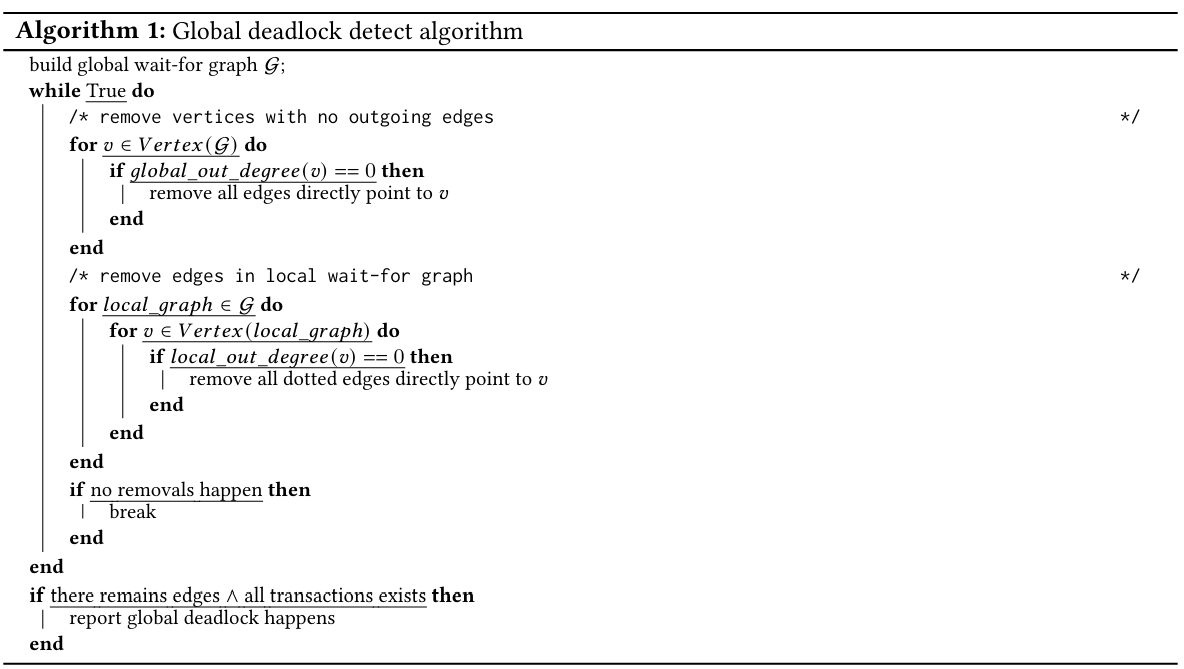
\includegraphics[width=1\linewidth]{algorithmGreenplum.png}
    \caption{Thuật toán global deadlock detect \cite{lyu2021Greenplum}}
    \label{fig:algorithmGreenplum}
\end{figure}

Giả sử trong một hệ thống cơ sở dữ liệu phân tán, các tiến trình A, B và C lần lượt đang chờ đợi các tài nguyên X, Y và Z. Quá trình này được biểu diễn bởi đồ thị chờ đợi toàn cầu. Khi tiến hành loại bỏ các đỉnh và cạnh, nếu phát hiện các tiến trình còn lại vẫn có mối quan hệ chờ đợi không thể giải quyết nhận định có deadlock.

Greenplum áp dụng một loạt các chiến lược để phát hiện, giải quyết và phòng ngừa deadlock, đảm bảo tính ổn định và hiệu suất của hệ thống.

Khi phát hiện deadlock, Greenplum đầu tiên sẽ xác định node để giải quyết tình trạng bế tắc. Node được chọn dựa trên một số tiêu chí như:Chi phí xử lý ưu tiên hủy những tiến trình có chi phí hoàn tác thấp nhất. Độ ưu tiên của tiến trình có độ ưu tiên thấp hơn có thể được chọn làm node xử lý. Thời gian hoạt động trong một số trường hợp, tiến trình đã hoạt động trong khoảng thời gian ngắn có thể được chọn để giảm thiểu tác động.

Tiến trình được chọn sẽ bị hủy, và tất cả tài nguyên đang giữ sẽ được giải phóng. Greenplum cũng sẽ ghi nhận trạng thái của tiến trình vào thời điểm hủy để giúp phục hồi dữ liệu nếu cần.

Sau khi hủy bỏ tiến trình, Greenplum có thể tự động khởi động lại tiến trình nếu cần thiết, đảm bảo rằng công việc không bị gián đoạn. Việc khởi động lại phải đảm bảo không tái tạo lại các điều kiện dẫn đến deadlock.

Để giảm thiểu nguy cơ phát sinh deadlock, Greenplum áp dụng một số biện pháp phòng ngừa:

Khóa hai giai đoạn (Two-Phase Locking)\cite{2pl}: Đảm bảo rằng mọi khoá phải được giữ cho đến khi giao dịch hoàn tất, ngăn ngừa các khoá được giải phóng sớm gây ra bế tắc.

Ưu tiên FIFO (First-In, First-Out): Điều này đảm bảo rằng các yêu cầu tài nguyên được xử lý theo thứ tự chúng được thực hiện, giảm thiểu khả năng xung đột.

Giám sát thời gian chờ đợi: Theo dõi thời gian chờ đợi của các tiến trình để phát hiện sớm các tình huống có thể dẫn đến deadlock.


